\chapter{Resultados}
\label{cap:Resultados}

En este capítulo se expondrán los resultados obtenidos a lo largo del desarrollo del proyecto, tras aplicar la metodología definida en el Capítulo \ref{cap:Metodologia}. De esta manera, se detallará en primer lugar una visión general del proyecto, compuesto por la planificación de las versiones, sus objetivos y el contexto en el que se enmarcan. Además, se desarrollará en este capítulo los sprints que se han llevado a cabo, junto con las funcionalidades que se han incluido en cada una de las versiones.

\section{Visión Global}
\label{sec:VisionGlobal}

Como se indicó anteriormente el OP de este proyecto consiste en el diseño y desarrollo de un JS de escritorio, cuyo aprovechamiento sirva para la enseñanza y el apoyo hacia aquellos usuarios que desean aprender conocimientos sobre el nuevo modelo de desarrollar software llamado DGS y en especial, como se lleva a cabo la labor de gestionar proyectos de estas características, utilizando técnicas de gamificación e inteligencia artificial.

\textbf{Grupo Objetivo}

El JS obtenido como resultado estará destinado en especial a estudiantes de ingeniería de software que desean aprender conocimientos sobre como se lleva a cabo el desarrollo de software en proyectos DGS, además de experimentar como llevar a cabo la gestión de este tipo de proyectos. Por otro lado, también estará dirigido a aquellos profesionales de la ingeniería del software que deseen ampliar sus conocimientos en otros modelos de desarrollar software, en especial con esta nueva tendencia, y así estar entrenados ante situaciones que puedan ocurrir en este tipo de proyectos y poder trabajar en un futuro en un entorno real.

\textbf{Necesidades}

La aparición de este nuevo modelo de desarrollo y la importancia que está tomando en los últimos años en el mundo laboral, hace necesaria la existencia de una buena educación y enseñanza de los aspectos y conceptos que lo engloban tanto en el ámbito estudiantil como en el laboral. Incluso, se añade la manifestación del fracaso de un gran número de proyectos con entornos globales debido, en especial mediada a su desconocimiento por parte de los miembros y a la difícil gestión que conlleva esta clase de proyectos, por lo que se hace necesario un entrenamiento previo.

\textbf{Producto}

Con este proyecto de TFG, se pretende obtener como resultado un JS de escritorio que permita a los jugadores jugar diferentes partidas, en donde el jugador (con el rol de jefe de proyecto) deberá gestionar un proyecto DGS ficticio, en el cual aparecerán múltiples situaciones o contratiempos que puedan ocurrir en un ambiente de estas características, las cuales deberán ser solventadas por el jugador.

\textbf{Beneficios}

Los beneficios que conlleva la utilización de esta herramienta consisten en el aprendizaje de un nuevo modelo de desarrollo de software, el cual está tomando cada vez más importancia y puede ser desconocido por un gran número de personas en la actualidad. Además, permite entrenarse en un escenario virtual conociéndose así las situaciones que puedan darse en un proyecto real de estas características, y poder afrontar con éxito la gestión del mismo.

El desarrollo del proyecto se ha dividido en tres versiones diferentes, las cuales serán definidas a continuación:

\begin{itemize}
	\item \textbf{Versión 1.} Esta primera versión se corresponderá con la redacción y definición de los requisitos iniciales del futuro JS. Además, se diseñaran los bocetos de las diferentes ventanas y vistas que poseerá la aplicación mediante la plataforma Balsamiq Mockup. Por otro lado, se llevará a cabo el estudio y aprendizaje de la herramienta para el desarrollo de videojuegos, Unity.
	\item \textbf{Versión 2.} Esta versión intermedia se centrará en el diseño de las diferentes interfaces gráficas de usuario de las cuales estará compuesta el juego, junto con el desarrollo del sistema para llevar a cabo una partida. Para ello se implementarán aspectos de gamificación y jugabilidad en el juego. Obtendremos como resultado una aplicación que nos permita jugar diferentes partidas al juego.
	\item \textbf{Versión 3.} Versión final de la aplicación la cual se centrará en la introducción de diferentes aspectos inteligentes sobre el juego, así como un sistema para la asignación de niveles y para poder llevar a cabo una enseñanza acorde con los conocimientos previos de cada usuario.
\end{itemize}

\section{Arquitectura}
\label{sec:Arquitectura}

A continuación, se detallará la arquitectura que se ha diseñado para conseguir el desarrollo de Global-Manager. Para ello, en este apartado se indican los componentes técnicos y funcionales del juego.

\subsection{Componentes técnicos}
\label{sec:ComponentesTecnicos}

En esta sección, se explicará la parte técnica que caracteriza a Global-Manager, es decir la arquitectura desarrollada para la construcción del juego. La arquitectura de la aplicación se puede desglosar en dos puntos de vista: lógico y software.

\subsubsection*{Arquitectura Lógica}

La arquitectura lógica está compuesta por todos los módulos que componen el juego, en la figura \ref{fig:ArquitecturaLogica} se puede observar la arquitectura lógica del JS.

% TODO: Insertar figura con los modulos del juego.

Los módulos expuestos en el juego son los siguientes:

\begin{itemize}
	\item \textbf{Módulo cuestionario:} Se compone de un conjunto de preguntas tipo test sobre conceptos relacionados con la gestión de proyectos y DGS que deben ser conocidas por un jefe de proyectos globales. Además, se pregunta al jugador sobre sus conocimientos, estudios y experiencias relacionadas con dichos temas. Este módulo se utiliza para crear un nuevo jugador en el sistema, para ello se expone al jugador a dicho cuestionario, con el fin de calcular un nivel de jugador y evaluar así sus conocimientos, proporcionándole una experiencia de juego acorde a sus capacidades.
	\item \textbf{Módulo configuración:} Contiene un conjunto de elementos y conceptos relacionados con la configuración inicial que se debe llevar a cabo en un proyecto de DGS, ayudando al jugador a familiarizarse con dichos conceptos. Con cada configuración del proyecto que se lleva a cabo, el juego calcula automáticamente en tiempo real un conjunto de factores de éxito para proporcionar al usuario si la configuración que está llevando a cabo es correcta o no. A su vez, se calcula un nivel de dificultad del proyecto. Por otro lado, para aquellos jugadores más inexpertos en el tema, se proporciona la opción de recalcular la configuración en función de su nivel de jugador.
	\item \textbf{Módulo juego:} Provee el sistema para ejecutar la partida del juego en función de la configuración del proyecto llevada a cabo. A lo largo de la partida, el módulo proporcionará diferentes eventos que el jugador deberá gestionar y solventar con éxito. El módulo evaluará el comportamiento del jugador y decidirá si ha adquirido nuevos conocimientos o necesita mejorar algunos aspectos.
	\item \textbf{Módulo interfaz:} Proporciona el medio para la interacción del estudiante con Global-Manager, a través de una interfaz gráfica de usuario. El diseño y desarrollo de la interfaz se ha llevado a cabo según los principios del diseño, implementación y evaluación de sistemas computacionales interactivos para su utilización por seres humanos, \emph{Human Computer Interaction} (HCI). De esta manera, se busca poner en práctica los procesos para la construcción de interfaces siguiendo el criterio de usabilidad, en el caso de los videojuegos, de jugabilidad.
\end{itemize}

\subsubsection*{Arquitectura Software}

La arquitectura software del JS está compuesto por un conjunto de capas en donde se dividen las componentes tecnológicas y software del juego utilizadas para su desarrollo. En la figura \ref{fig:ArquitecturaSoftware} se puede observar la arquitectura software de Global-Manager.

\begin{figure}[htb]
	\centering
	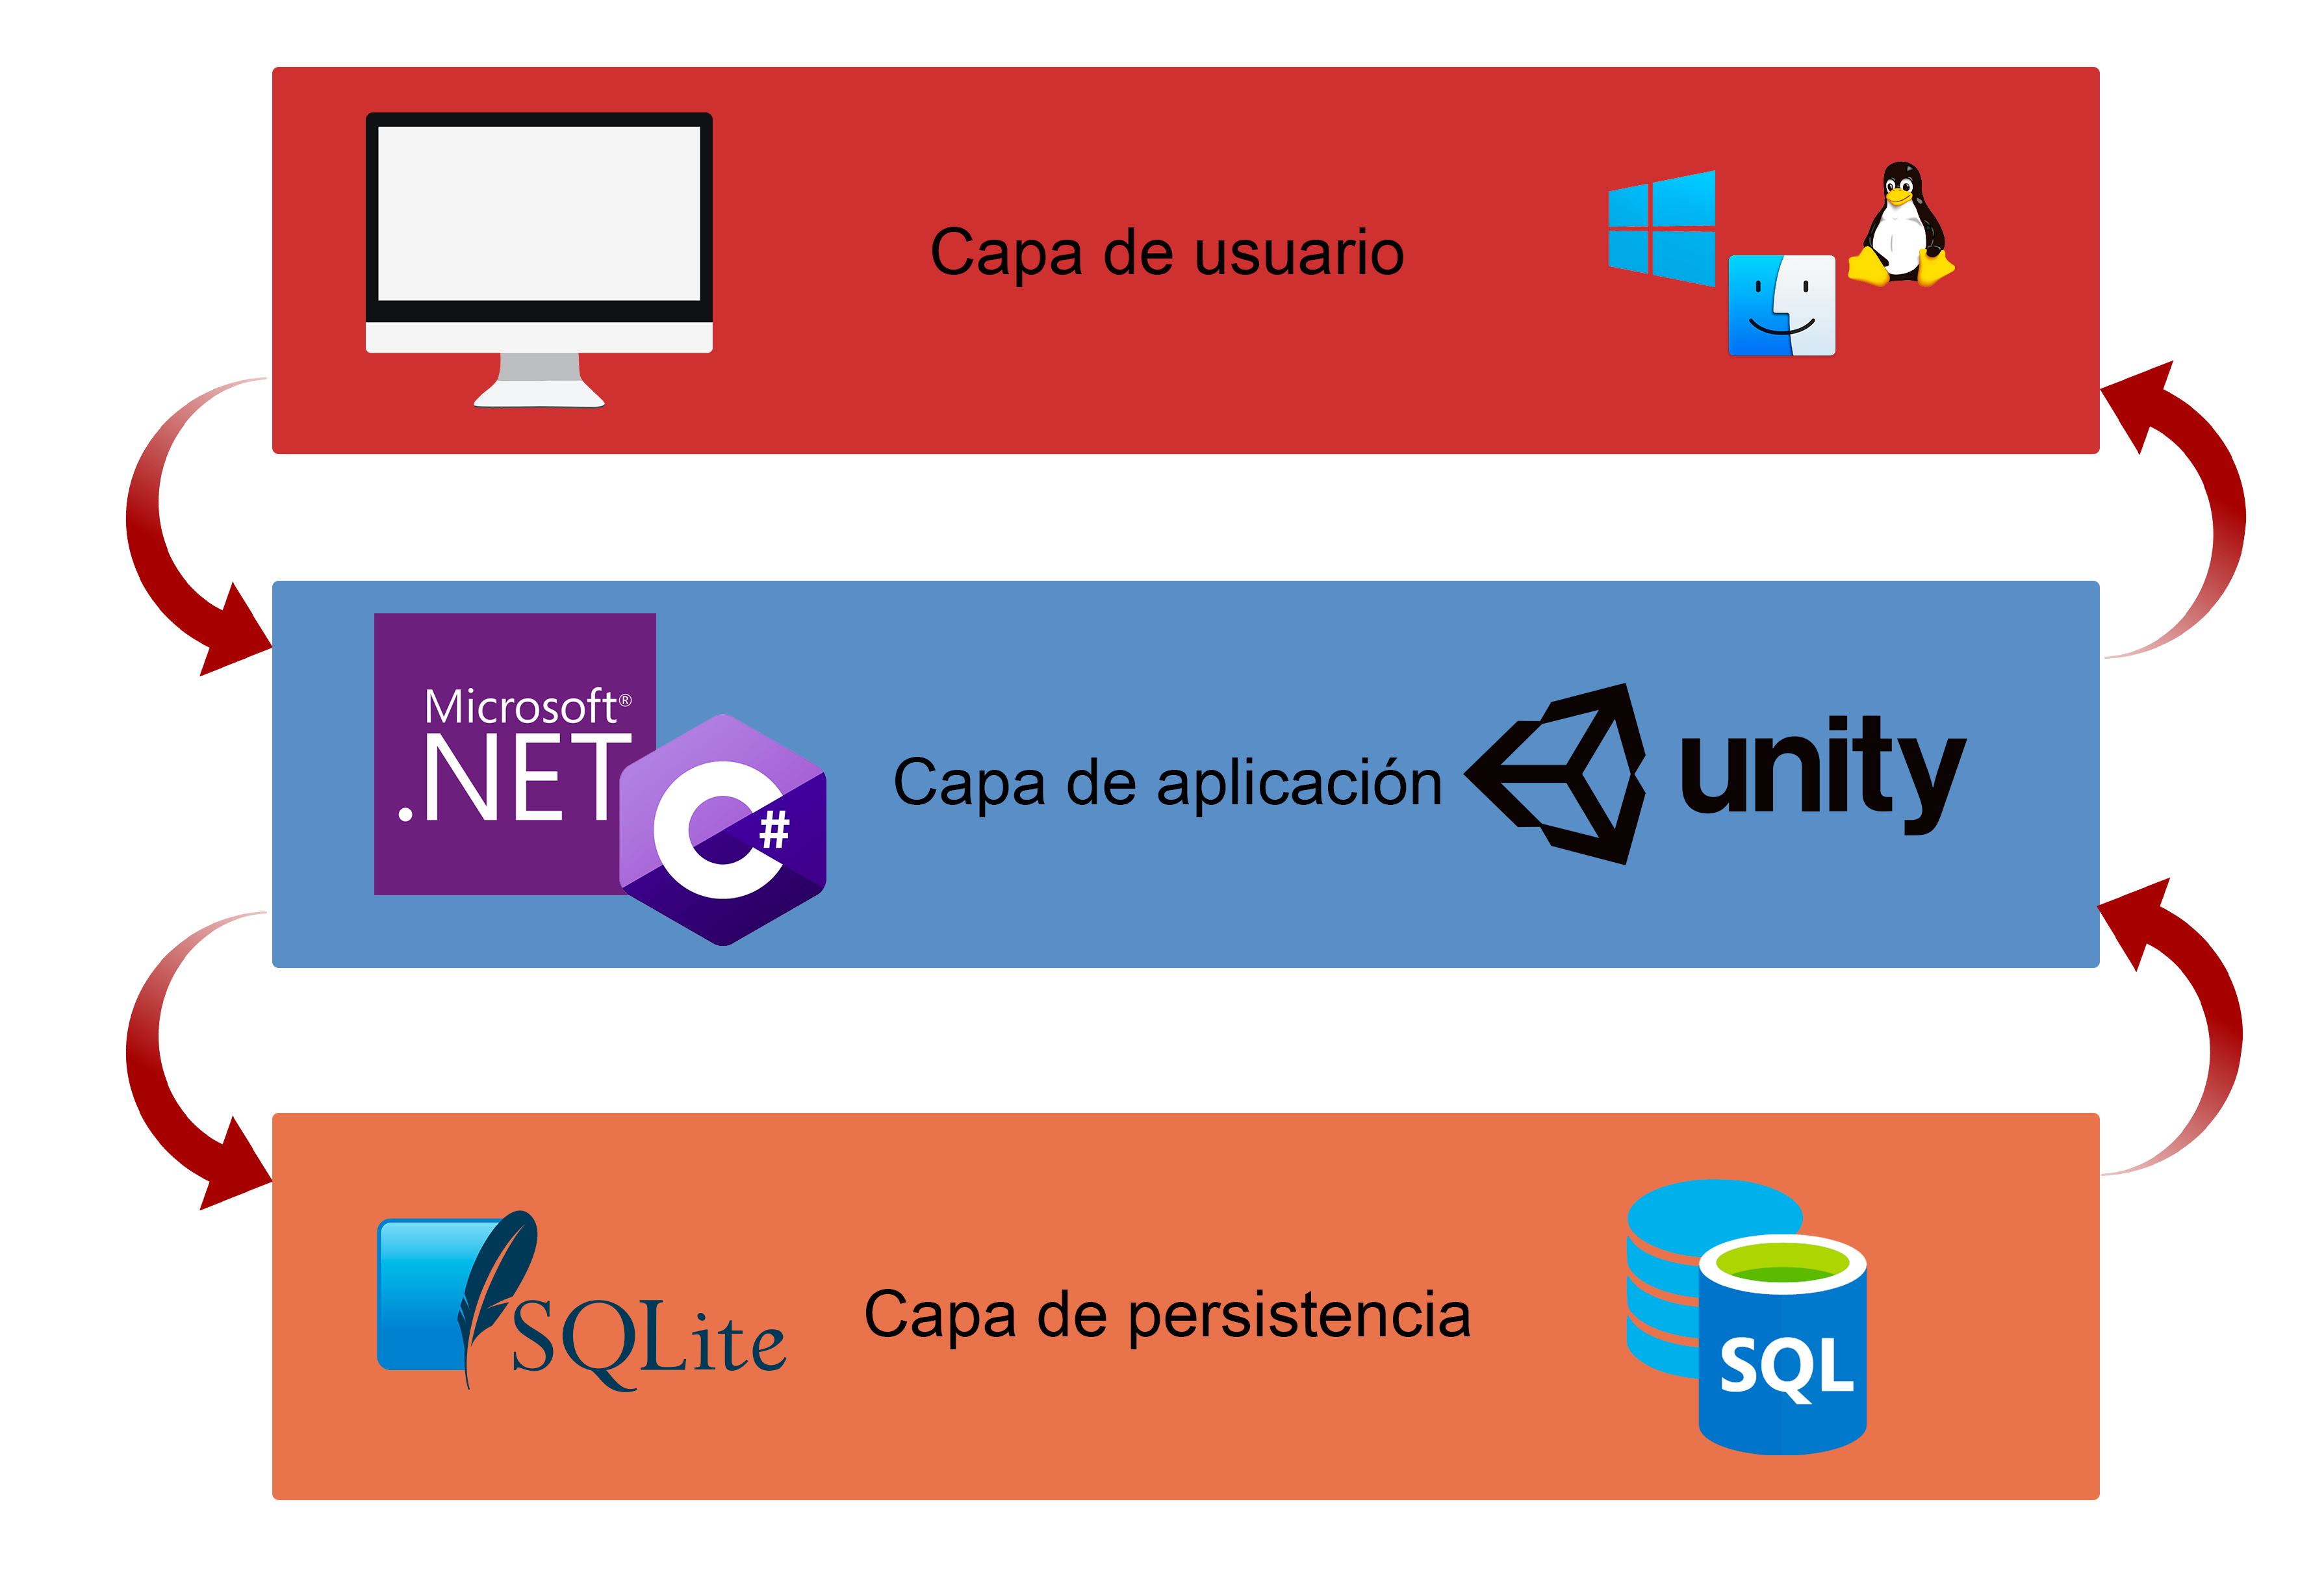
\includegraphics[width=0.95\linewidth]{ArquitecturaSoftware}
	\caption[Arquitectura software de Global-Manager]{Arquitectura software de Global-Manager}
	\label{fig:ArquitecturaSoftware}
\end{figure}

Esta arquitectura software esta compuesta por tres capas:

\begin{itemize}
	\item \textbf{Capa de usuario.} Representa el entorno sobre el cual se podrá ejecutar la aplicación. En nuestro caso, el JS consistirá en una aplicación de escritorio, la cual se podrá ejecutar en los sistemas operativos \emph{Windows}, \emph{Linux} y \emph{Mac OS}.
	\item \textbf{Capa de aplicación.} Consiste en la capa que hace referencia al JS, el cual consistirá en un proyecto \emph{.NET Framework}, en el cual se utiliza el motor de videojuegos y físicas, \emph{Unity} junto con diferentes \emph{scripts} escritos en el lenguaje de programación C\#.  
	\item \textbf{Capa de persistencia.} Esta última capa hace referencia a la base de datos o modelo de datos, donde se almacenará toda la información relevante tanto de la aplicación como de los usuarios. Para ello, se ha optado por utilizar como motor de base de datos \emph{SQLite}, de esta manera existirá una base de datos SQLite en local y se llevará a cabo el intercambio de información mediante sentencias SQL.
\end{itemize}

\subsection{Componentes funcionales}
\label{sec:ComponentesFuncionales}

A continuación, se presentará una visión global del funcionamiento del juego, a través de un flujo de ejecución del juego:

\begin{enumerate}
	\item Al empezar el juego y si el jugador nunca ha jugado, este deberá rellenar un cuestionario para registrar un nuevo jugador en el sistema y obtener un nivel de usuario.
	\item Si el jugador ya tiene almacenado en el sistema un jugador, este podrá comenzar una partida seleccionando el jugador con el que desea jugar.
	\item Una partida comenzará con la ventana de configuración del proyecto, en ella, el jugador configurará un proyecto global a su gusto seleccionando y rellenando todos los componentes que aparecen en pantalla. En caso de que el jugador no sepa (debido a su bajo nivel de conocimientos) o no quiera configurar un nuevo proyecto, podrá solicitar una configuración de proyecto recomendada automáticamente en función de su nivel de jugador. Una vez, el proyecto este configurado, el jugador podrá comenzar la fase de juego.
	\item Una vez que empiece la fase de juego, se llevará a cabo una simulación de un proyecto de global y el módulo de juego proporcionará diferentes eventos que el jugador, en el rol de jefe de proyecto, deberá hacer frente y solventar.
	\item Un partida terminará exitosamente cuando se consiga la finalización del proyecto con la entrega del producto al cliente, o sin embargo, cuando el proyecto se quede sin presupuesto o no se llegue a tiempo a entregar el producto.
	\item Al finalizar la partida, el sistema proporcionara un registro con el resultado de la partida y una evaluación con el comportamiento del jugador.
	\item El jugador podrá volver a empezar otra partida.
\end{enumerate}

\section{Hoja de ruta}
\label{sec:HojaRuta}

A continuación, se muestra en la tabla \ref{tab:Versiones} el conjunto de todas las versiones desarrolladas a lo largo del proyecto junto con una breve descripción de sus funcionalidades.

%TODO: Añadir tabla con las versiones del juego

\section{Versión Key}
\label{sec:VersionKey}

Esta versión se corresponde con la fase inicial del proyecto, en donde se aborda la preparación del proyecto, se adquieren los conocimientos necesarios y se comienza con el diseño del proyecto.

\subsection{Contexto}
\label{sec:ContextoKey}

Uno de los grandes problemas al que había que enfrentarse al comienzo de este proyecto era el absoluto desconocimiento de las tecnologías seleccionadas para llevar a cabo el desarrollo del juego, por un lado, del lenguaje de programación C\# y por otro, de la herramienta de desarrollo de videojuegos, \emph{Unity}.

Por esta razón, era notoria la necesidad de adquirir los conocimientos necesarios para saber utilizar correctamente dicho entorno de desarrollo y lenguaje de programación. Para ello, se realizó un curso de \emph{Domestika} \footnote{\url{https://www.domestika.org/es}} sobre el desarrollo de videojuegos 3D en Unity. Además, a través de los cursos de \emph{SoloLearn}, se realizó aquel para aprender a manejar el lenguaje de programación C\#.

Del mismo modo, también se procedió con el diseño de los bocetos iniciales de las ventanas del juego utilizando la herramienta para la creación de bocetos software, \emph{Balsamiq Mockup}. En especial, se diseñaron las ventanas de configuración del proyecto y juego.

\subsection{Temporización}
\label{sec:TemporizacionKey}

La versión Key esta compuesta de un total de cuatro \emph{sprints}, los cuales se corresponden con los primeros sprints del proyecto. La fase de desarrollo de dicha versión ocupó los meses de Marzo y Abril de 2020, a continuación se describen los detalles de la fase:

\begin{enumerate}
	\item \textbf{Sprint 1 (Curso SoloLearn):} Este primer sprint sirvió para llevar a cabo el curso de SoloLearn sobre el lenguaje de programación C\#, el cual nos aporto los conocimientos necesarios para manejar dicho lenguaje: conceptos básicos, bucles y condicionales, métodos, clases y objetos, arrays, strings, structs, enums, exceptiones, dictionaries and lists.
	\item \textbf{Sprint 2 (Curso Domestika):} En este segundo sprint, después de haber aprendido a manejar el lenguaje de programación C\#, se procedió a llevar a cabo el curso de Domestika, donde se obtienen los conocimientos necesarios para crear videojuegos en 3D desde cero a través de la plataforma Unity. En dicho curso se abordaron los siguientes temas: conceptos básicos, propiedades de un proyecto, manejo de personajes y colisiones, iluminación, prefabs e inteligencia artificial, e interfaz de usuario.
	\item \textbf{Sprint 3 (Boceto ventana de configuración del proyecto):} Una vez hemos aprendido las herramientas necesarias para llevar a cabo el proyecto, se comenzó con el desarrollo del proyecto, en especial y en primer lugar, con el diseño de los bocetos del futuro JS. En este sprint, se procedió con el diseño inicial de la ventana de configuración del proyecto a través de la herramienta de prototipado de interfaces gráficas de usuario, Balsamiq Mockups.
	\item \textbf{Sprint 4 (Boceto ventana de juego):} Al igual que en el sprint anterior, se llevó a cabo el diseño de la interfaz gráfica de usuario y de la disposición de los objetos en la fase de juego. 
\end{enumerate}

\begin{figure}[htb]
	\centering
	\includegraphics[width=1\linewidth]{GanttVersiónKey}
	\caption[Diagrama de Gantt de los sprints de la versión Key]{Diagrama de Gantt de los sprints de la versión Key}
	\label{fig:GanttVersionKey}
\end{figure}

\subsection{Bocetos de Global-Manager}
\label{sec:BocetosGlobal-Manager}

Como se ha indicado en el apartado anterior, en esta versión se han diseñado los bocetos, sobre los cuales se desarrollarán las interfaces gráficas de usuario del juego, en especial, de las ventanas principales: configuración del proyecto y fase de juego. Se realizaron varios bocetos con el fin de conseguir el mejor diseño posible, garantizando una correcta usabilidad. Junto con la co-tutora de este TFG, Aurora Vizcaíno Barceló se evaluaron y mejoraron los bocetos, hasta conseguir los diseños finales. A continuación, se muestran dichos bocetos junto con una breve descripción, ya que dichos diseños serán explicados posteriormente en detalle en las versiones correspondientes donde se llevó a cabo el desarrollo de dichas interfaces gráficas dentro de la plataforma Unity.

\subsubsection*{Boceto de configuración del proyecto}
\label{BocetoConfiguracionProyecto}

En primer lugar, cuando el jugador comience una partida tendrá la ventana de configuración del proyecto. A continuación, en la figura \ref{fig:VentanaConfiguracionBoceto}, se muestra el boceto final del diseño de la interfaz gráfica para la configuración de un proyecto, antes de empezar la fase de juego.

\begin{figure}[htb]
	\centering
	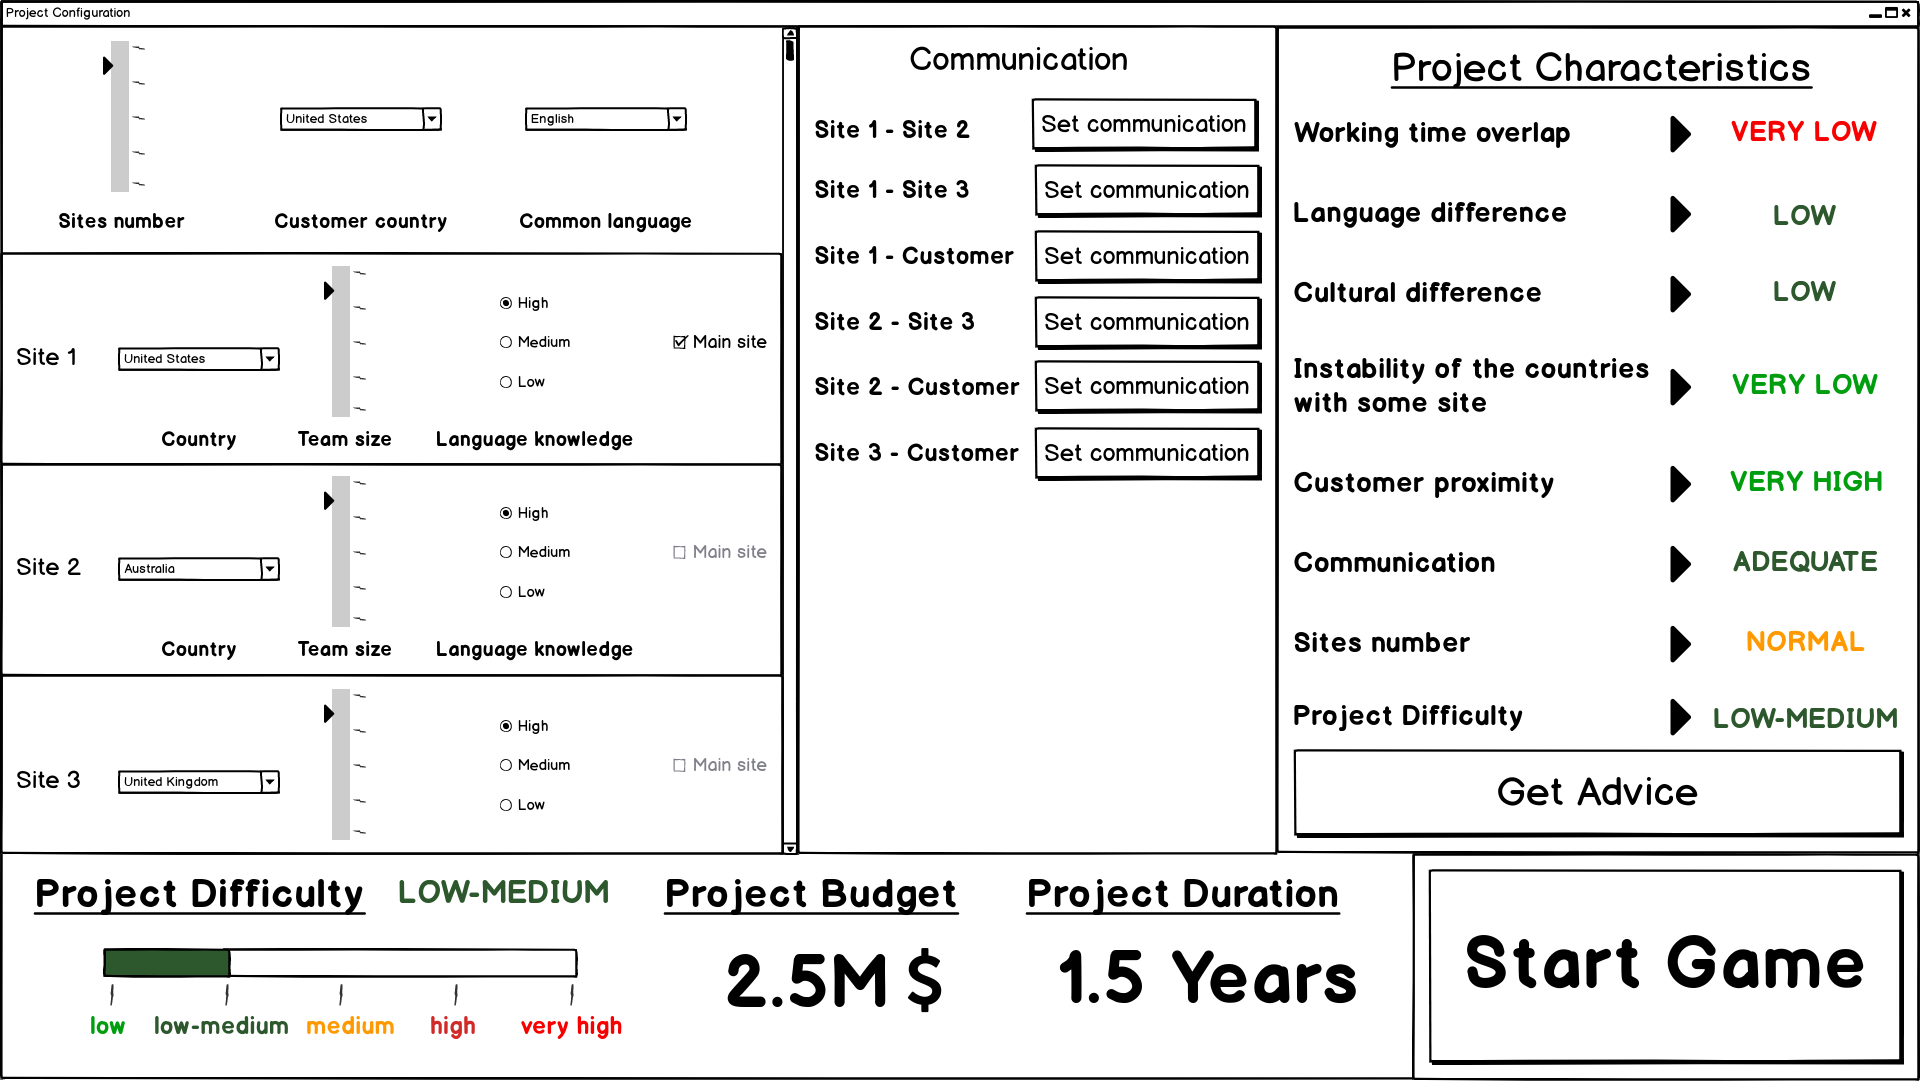
\includegraphics[width=0.95\linewidth]{VentanaConfiguracionBoceto}
	\caption[Boceto de la ventana de configuración del proyecto]{Boceto de la ventana de configuración del proyecto}
	\label{fig:VentanaConfiguracionBoceto}
\end{figure}

Como se puede observar, se ha optado por un diseño, en el cual, los elementos relacionados con la configuración del proyecto se mantengan en todo momento en pantalla, mientras el jugador interacciona con ellos. De esta manera, conseguimos que el jugador analice todos los elementos a configurar de un vistazo. Los parámetros que tienen que ser configurados están relacionados con conceptos básicos y componentes característicos de un proyecto de DGS, como pueden ser: el número de sites del proyecto, el país donde se ubica tanto el cliente como los demás equipos de trabajo, el número de trabajadores por cada equipo de trabajo, el idioma principal de comunicación entre los miembros del proyecto o la ubicación del site principal de desarrollo del proyecto. Por otro lado, el jugador también configurará las herramientas con las que se comunicarán cada uno de los equipos de trabajo del proyecto. Además, en la interfaz se mostrarán un conjunto de características referentes a un proyecto global y se indicará mediante el uso de etiquetas lingüísticas su valoración en el proyecto configurado. Con ello, también se mostrará la dificultad de llevar a cabo la gestión del proyecto con dicha configuración. Cabe destacar, que se proporcionará un botón para obtener recomendaciones que nos indiquen que parámetros se deben cambiar para reducir la dificultad del proyecto, destinado a aquellos jugadores menos experimentados. Otra información relevante como la duración o el presupuesto inicial del proyecto también se presentan en esta interfaz.

Con este boceto, perseguimos que el jugador adquiera y se familiarice con los conceptos y elementos básicos de los proyectos DGS, aprenda como estos elementos modifican las características del proyecto y su dificultad, y conozca que configuraciones de proyectos son más fáciles de gestionar y cuales más complicadas. 

\subsubsection*{Boceto fase de juego}
\label{BocetoFaseJuego}

Por otro lado, una vez el jugador configura un proyecto, se procederá con la fase de juego. En esta parte de la partida, se lleva a cabo una simulación del proyecto DGS configurado. En la figura \ref{fig:VentanaJuegoBoceto}, se puede observar el boceto de la interfaz de juego.

\begin{figure}[htb]
	\centering
	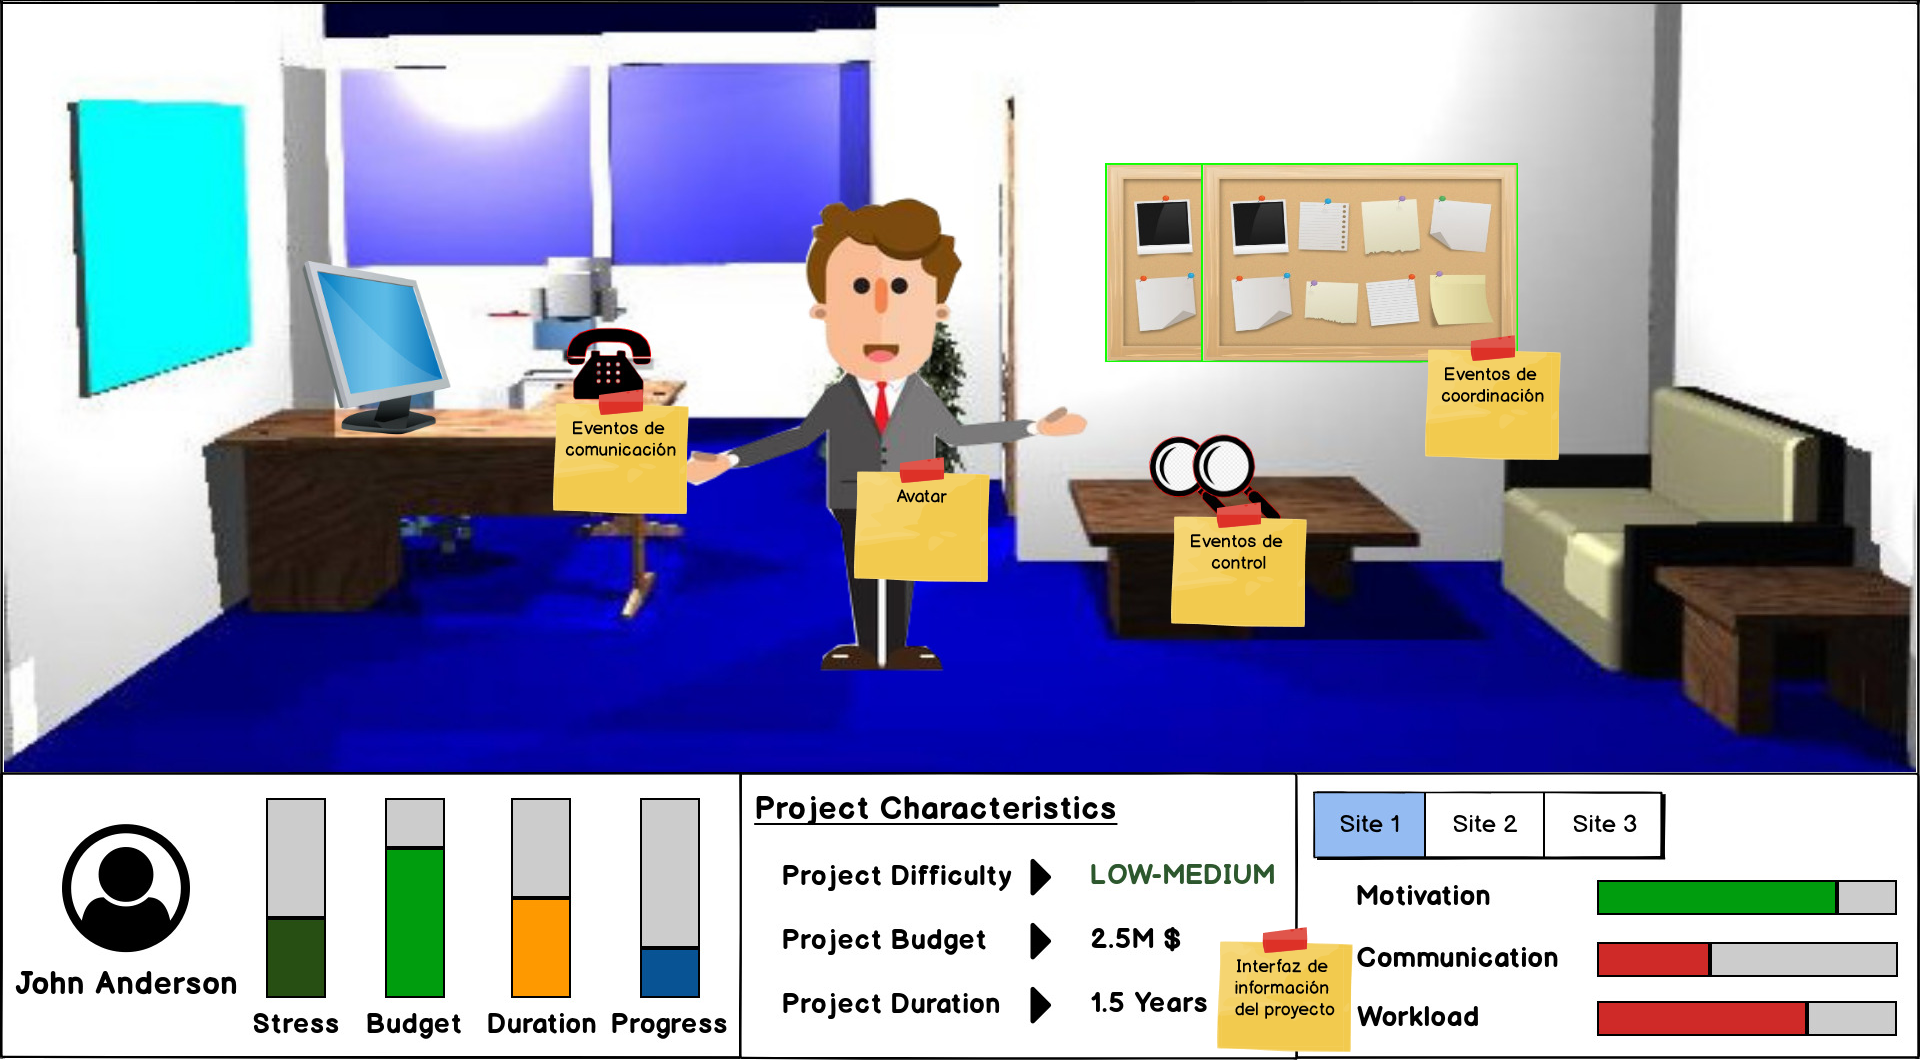
\includegraphics[width=0.95\linewidth]{VentanaJuegoBoceto}
	\caption[Boceto de la ventana de juego]{Boceto de la ventana de juego}
	\label{fig:VentanaJuegoBoceto}
\end{figure}

En esta ventana, aparecería el entorno de juego, el cual se correspondería con el de una oficina, junto con un avatar del personaje, el cual representaría al jugador. En este escenario, descenderían diferentes objetos, los cuales representarían situaciones o eventos que pueden ocurrir en estos proyectos. Estos eventos podrán ser buenos, con una repercusión positiva en el proyecto o malos, en cuyo caso consistirían en impedimentos (representados a través de una pregunta) ocurridos en el proyecto y el jugador, en el rol de jefe de proyecto, deberá solventar dicha situación escogiendo la mejor opción (mejor respuesta entre varias). Estos eventos hacen referencia a los tres grandes desafíos de los proyectos DGS: teléfono (comunicación), post-it (coordinación) y lupa (control). Por otro lado, en la parte inferior de la ventana aparecería información relevante sobre el proyecto que se está gestionando, como el estrés del jugador, el presupuesto, la duración o el progreso actual del proyecto que se representaría a través de barras de progreso; información inicial como dificultad, presupuesto o duración inicial; e información sobre cada uno de los sites como motivación, comunicación con los demás sites o carga de trabajo, representado mediante barras de progreso.

De esta manera, buscamos que el jugador se sienta en la piel de un jefe de proyecto DGS y aprenda a hacer frente las dificultades que conlleva gestionar esta clase de proyectos, en especial los relacionados con la comunicación, coordinación y control.

\section{Versión Design}
\label{sec:VersionDesign}

Después de haber aprendido los conocimientos necesarios para manejar el entorno de desarrollo de videojuegos Unity, habría que comenzar a desarrollar el JS. En esta versión, se comienza a desarrollar las interfaces gráficas de usuario de las ventanas de cuestionario de nivel y configuración del proyecto. 

\subsection{Temporización}
\label{sec:TemporizacionDesign}

En esta nueva versión, se realizaron los correspondientes sprints 6 y 7, los cuales tuvieron lugar durante el mes de Mayo de 2020. A continuación, se expresa una breve descripción de cada sprint:

\begin{enumerate}
	\item \textbf{Sprint 6 (Diseño cuestionario de nivel):} Este sprint comienza el desarrollo del JS, Global-Manager, desarrollándose una ventana gráfica en donde el jugador pueda crear y almacenar un nuevo usuario con el cual poder jugar. Esta ventana también servirá para asociarle al jugador un nivel de jugador, a través del cual se identifique el nivel de conocimiento del jugador. Es por esto, que en dicha interfaz se ha incorporado un cuestionario con diferentes preguntas sobre el tema, a través del cual sea posible calcular los conocimientos actuales del jugador.
	\item \textbf{Sprint 7 (Diseño configuración del proyecto):} Con el diseño de la interfaz de cuestionario de nivel desarrollado, se procedió con el diseño de la ventana de configuración del proyecto, utilizando como ejemplo el boceto diseñado en la versión anterior. 
\end{enumerate}

\begin{figure}[htb]
	\centering
	\includegraphics[width=1\linewidth]{GanttVersiónDesign}
	\caption[Diagrama de Gantt de los sprints de la versión Design]{Diagrama de Gantt de los sprints de la versión Design}
	\label{fig:GanttVersionDesign}
\end{figure}

\subsection{Diseño cuestionario de nivel}
\label{sec:DiseñoCuestionarioNivel}

En primer lugar, para iniciar la creación del juego, se ha comenzado con el desarrollo del diseño de una interfaz con la cual el jugador, si no posee ningún perfil almacenado en el juego, pueda crearse uno nuevo. A través de este perfil de jugador, se podrá llevar a cabo un seguimiento de las partidas realizadas y evaluar como evoluciona su flujo de aprendizaje. Por otro lado, mediante esta interfaz se pretende calcular los conocimientos actuales del jugador sobre DGS y gestión de proyectos y obtener de esta manera un nivel de jugador que nos indique el grado de conocimiento. Para llevar a cabo dicho cálculo, se utilizará un cuestionario con diferentes preguntas sobre la experiencia del jugador, conocimiento que posea y conceptos básicos de DGS y gestión de proyectos. De esta manera, el jugador rellenará el cuestionario con el objetivo de crear un perfil, pero también se evaluarán sus conocimientos para obtener un nivel de jugador y ofrecer una experiencia de usuario acorde a sus conocimientos. 

Para componer el cuestionario para el cálculo del nivel de jugador, nos apoyamos en una pequeña entrevista realizada a la experta en DGS y co-tutora de este TFG, Aurora Vizcaíno Barceló, con el objetivo de conocer cuales son las componentes que se deben tener en cuenta para extraer el grado de conocimiento de una persona en dicho tema. Además de las preguntas extraídas de la entrevista, se añadieron algunas más, variación de las ya obtenidas. A continuación en la figura \ref{fig:VentanaCuestionarioNivel}, se muestra el resultado final de la interfaz gráfica de la ventana cuestionario de nivel, con el conjunto de preguntas seleccionadas.

\begin{figure}[htb]
	\centering
	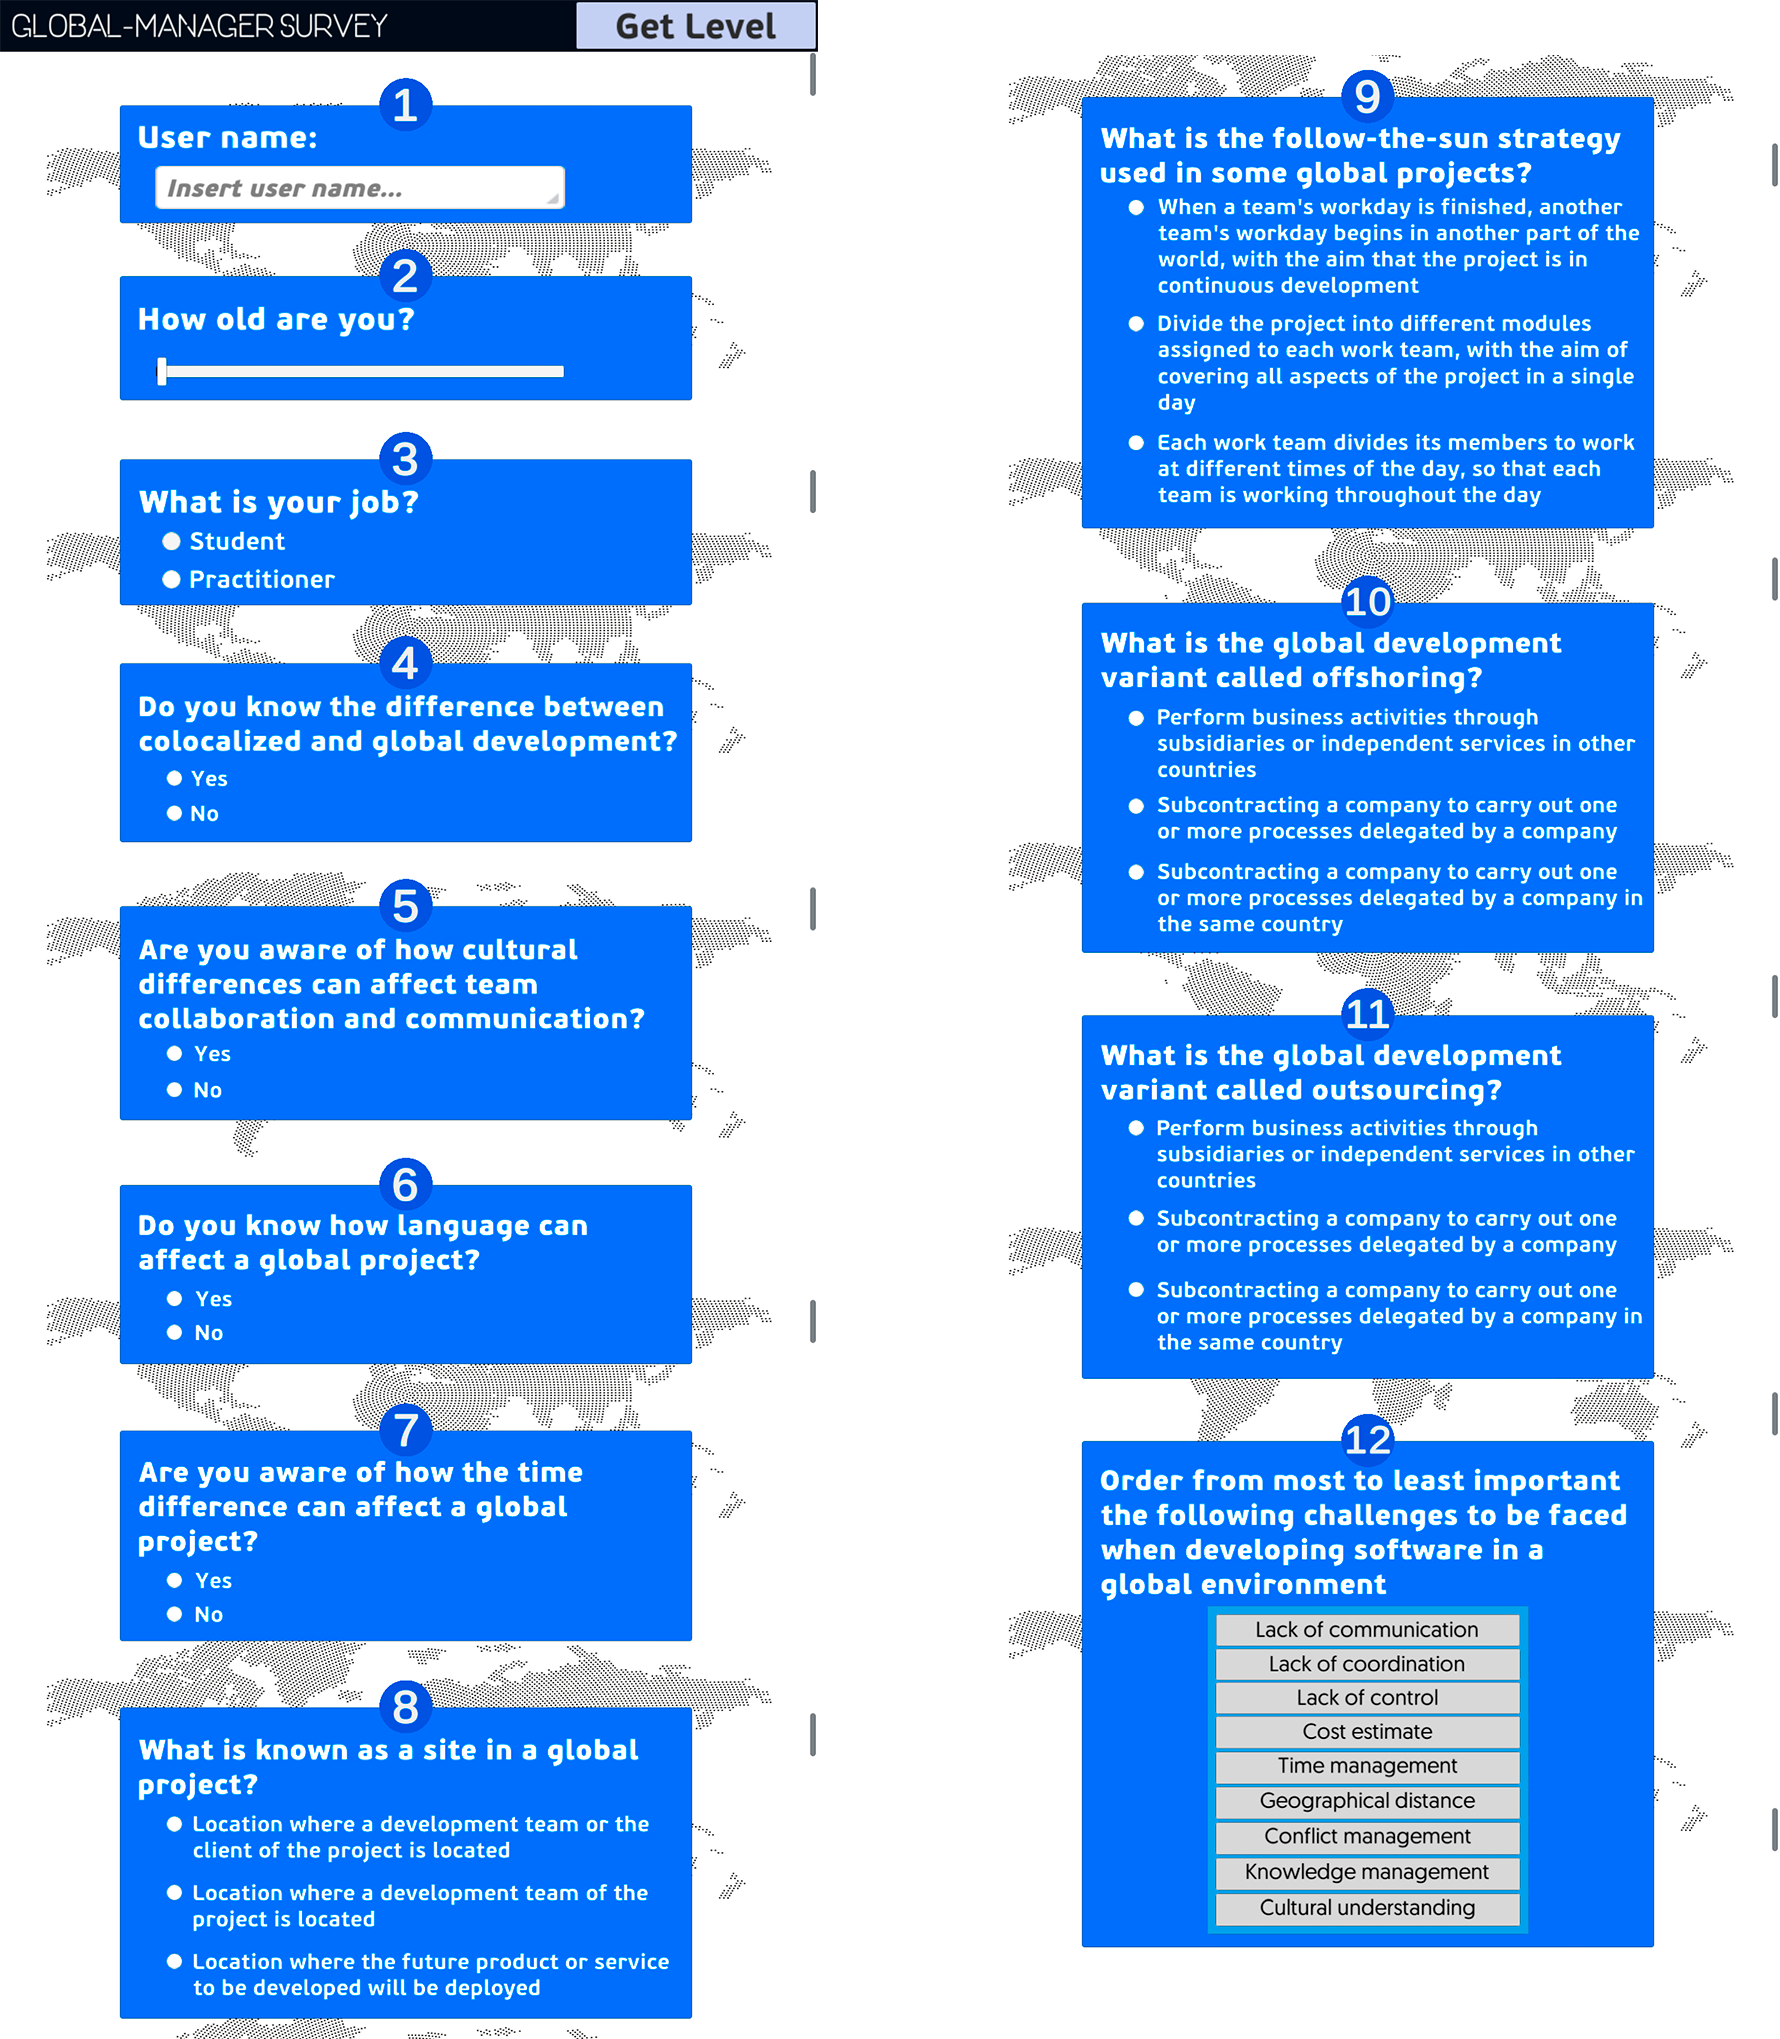
\includegraphics[width=1\linewidth]{VentanaCuestionarioNivel}
	\caption[Ventana del cuestionario de nivel]{Ventana del cuestionario de nivel}
	\label{fig:VentanaCuestionarioNivel}
\end{figure}

Como se puede observar, el cuestionario consta de un total de doce cuestiones generales, donde la mayoría de ellas se corresponden con preguntas tipo test. Las dos primeras preguntas aluden a información relevante del jugador, como es el nombre de usuario que se desea tener y la edad que posee. Seguidamente, se encontrarán un total de nueve preguntas tipo test, las cuales podemos dividir en tres grandes grupos:

\begin{itemize}
	\item \textbf{Pregunta 3:} Se corresponde con una pregunta utilizada para conocer la situación actual del jugador, es decir, si se encuentra estudiando o trabajando profesionalmente en el mercado, dependiendo de la respuesta, se realizarán al final del cuestionario una clase de preguntas diferentes. En el caso de que la respuesta sea estudiante (\emph{Student}), se mostrarán las preguntas de la figura \ref{fig:PreguntasStudent}, de igual manera, si la respuesta fuese profesional (\emph{Practitioner}), las preguntas mostradas serían las de la figura \ref{fig:PreguntasPractitioner}.
	\item \textbf{Preguntas 4-7:} Consisten en un conjunto de cuestiones tipo test donde las respuestas son: sí poseo los conocimientos (\emph{Yes}), y no poseo los conocimientos (\emph{No}). Estas cuestiones sirven para conocer los conocimientos actuales que posee el jugador del tema de DGS y gestión de proyectos en relación con \emph{diferencia entre desarrollo colocalizado y global}, \emph{diferencia cultural}, \emph{desigualdad lingüística} y \emph{disparidad horaria} en un proyecto global.
	\item \textbf{Preguntas 8-11:} Se corresponden con un conjunto de preguntas tipo test sobre elementos y conceptos básicos sobre la gestión en proyectos de software globales. Estas preguntas hacen referencia a los conceptos de: \emph{site}, \emph{estrategia follow-the-sun}, \emph{offshoring} y \emph{outsourcing}. A continuación, se muestra una traducción de cada pregunta junto con su respuesta correcta:
	\begin{itemize}
		\item \textbf{¿Qué es lo que se conoce como un site en un proyecto global?} Ubicación donde se encuentra un equipo de desarrollo del proyecto.
		\item \textbf{¿Qué es la estrategia follow-the-sun utilizada en algunos proyectos globales?} Cuando un equipo de trabajo acaba su jornada laboral, la jornada de otro equipo comienza en otra parte del mundo, con el objetivo de que el proyecto este en constante desarrollo.
		\item \textbf{¿Qué es la variante de desarrollo global llamada offshoring?} Realizar actividades de negocio a través de filiares o servicios independientes en otros países.
		\item \textbf{¿Qué es la variante de desarrollo global llamada outsourcing?} Subcontratar una compañía para llevar a cabo uno o más procesos delegados por la compañía.
	\end{itemize}
\end{itemize}

Prosiguiendo, en la siguiente cuestión (pregunta 12), se le pide al jugador que ordene de más a menos importante un conjunto de desafíos, que se pueden encontrar en entornos DGS. El orden correcto de la respuesta a esta pregunta, según el estudio realizado en \cite{niazi2016challenges} y la tabla \ref{tab:DificultadesDGS}, donde se citan los desafíos más importantes en los proyectos DGS, sería: \emph{cultural understanding}, \emph{lack of communication}, \emph{knowledge management}, \emph{time management}, \emph{lack of coordination}, \emph{lack of control}, \emph{conflict management}, \emph{cost estimate} y \emph{geographical distance}.

Por último, en función de la respuesta indicada del jugador en la pregunta 3, se mostrarán dos preguntas adicionales de tipo test con respuestas de \emph{Yes} y \emph{No}. En el caso de indicar el jugador que es estudiante, se mostrarán las preguntas de la figura \ref{fig:PreguntasStudent}, para conocer si ha estudiado DGS o gestión de proyectos. En caso contrario, si el jugador ha indicado que es profesional, se indicarán las preguntas de la figura \ref{fig:PreguntasPractitioner}, para conocer si alguna vez ha trabajado en un proyecto global o como jefe de proyecto.

\begin{figure}[htb]
	\centering
	\begin{subfigure}[b]{1\linewidth}
		\centering
		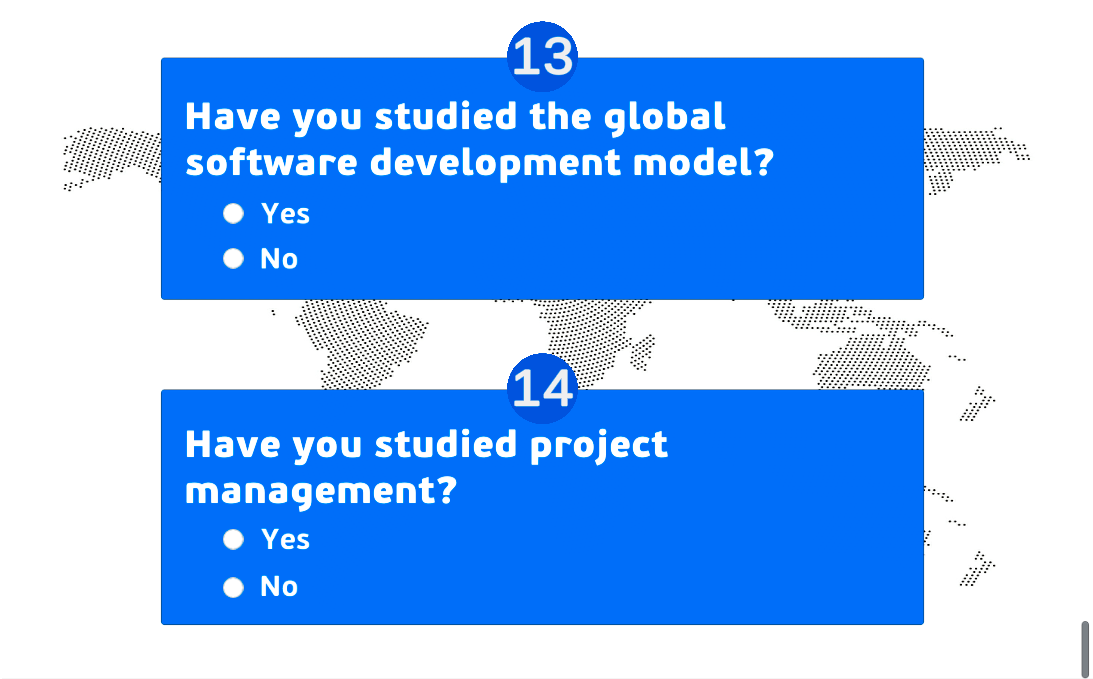
\includegraphics[width=0.8\linewidth]{PreguntasStudent}
		\caption{Preguntas para los estudiantes}\label{fig:PreguntasStudent}
	\end{subfigure}
	\begin{subfigure}[b]{1\linewidth}
		\centering
		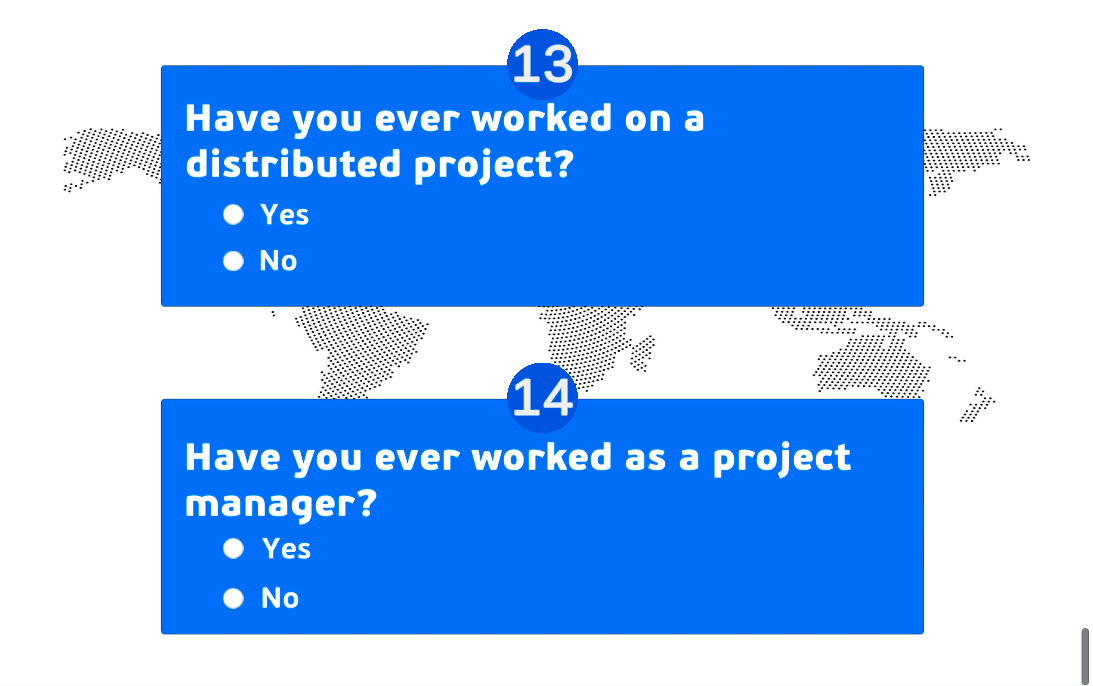
\includegraphics[width=0.8\linewidth]{PreguntasPractitioner}
		\caption{Preguntas para los profesionales}\label{fig:PreguntasPractitioner}
	\end{subfigure}
	\caption[Preguntas especializadas para estudiantes y profesionales]{Preguntas especializadas para estudiantes y profesionales}
	\label{fig:PreguntasAdicionales}
\end{figure}

\subsection{Diseño configuración del proyecto}
\label{sec:DiseñoConfiguracionProyecto}

Una vez se ha desarrollado el diseño para la ventana cuestionario de nivel, donde se muestra un pequeño cuestionario con el cual el jugador puede crear y almacenar un nuevo usuario, y obtener un nivel de jugador acorde a sus conocimientos en el tema; es necesario comenzar a desarrollar la ejecución de las partidas. Para ello comenzaremos con el desarrollo del diseño de la ventana de configuración del proyecto, permitiendo al jugador interactuar con diferentes elementos relacionados con la configuración de un proyecto de software global.

El diseño de la interfaz gráfica de la ventana de configuración del proyecto se puede observar en la siguiente figura \ref{fig:ConfigurationWindow}. La disposición del diseño de la ventana se puede dividir en siete partes diferentes: \emph{configuración inicial}, \emph{configuración de sites}, \emph{configuración de la comunicación}, \emph{características del proyecto}, \emph{presupuesto y duración}, \emph{dificultad del proyecto}, \emph{botón de empezar partida}.

\begin{figure}[htb]
	\centering
	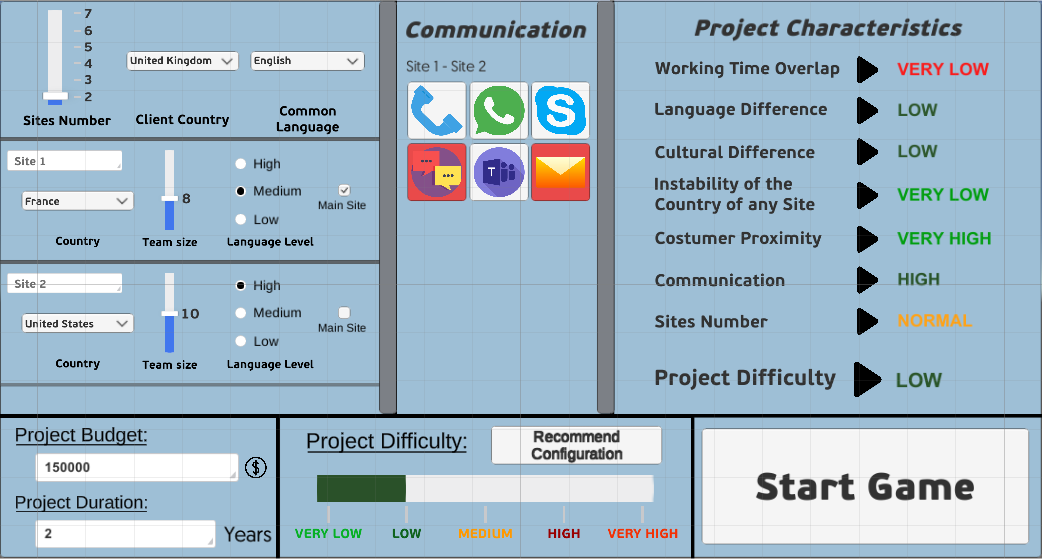
\includegraphics[width=0.95\linewidth]{ConfigurationWindow}
	\caption[Diseño de la ventana de configuración de un proyecto global]{Ventana de configuración del proyecto}
	\label{fig:ConfigurationWindow}
\end{figure}

A continuación, se indicará una pequeña descripción de cada una de las partes de la ventana de configuración del proyecto:

\begin{itemize}
	\item \textbf{Configuración inicial:} Corresponde a los primeros parámetros que el jugador debe de configurar, estos son: el número de sites (2-7) que compondrá el proyecto (mediante un slider), el país donde se encuentra el cliente (mediante un combo box) y el idioma con el que se comunicarán los diferentes miembros del proyecto (mediante un combo box).
	\item \textbf{Configuración de sites:} En función del número de sites definido anteriormente, se mostrará un cuadrado por cada site. El jugador deberá establecer los diferentes parámetros necesarios para cada site. Estos parámetros son: un nombre que lo distinga de los demás (mediante un campo de entrada), el país donde se encuentra el site (mediante un combo box), el tamaño del equipo de trabajo (2-20 miembros), el nivel del idioma definido anteriormente como idioma global del proyecto (se muestra mediante tres botones las opciones, \emph{high}, \emph{medium} y \emph{low}) y por último, el jugador indicará mediante el botón correspondiente a dicho site, aquel que se corresponda con el site central del proyecto.
	\item \textbf{Configuración de la comunicación:} Con el número de sites definido anteriormente, se mostrarán todas las combinaciones posibles entre los diferentes sites y el jugador tendrá que seleccionar mediante botones aquellas herramientas de comunicación que se utilizarán para llevar a cabo el intercambio de información en cada una de las combinaciones. Las herramientas de comunicación son las siguientes: \emph{teléfono}, \emph{WhatsApp}, \emph{Skype}, \emph{foros}, \emph{Microsoft Teams} y \emph{e-mail}.
	\item \textbf{Características del proyecto:} Se muestran un conjunto de características del proyecto o factores de éxito junto con la dificultad del proyecto. Estas características son recalculadas automáticamente en tiempo real en función de la configuración del proyecto actual realizada por el jugador. Estas caracteristicas poseen unas etiquetas lingüísticas para darles valor, estas son: \emph{VERY LOW}, \emph{LOW}, \emph{NORMAL}, \emph{HIGH} y \emph{VERY HIGH}. Estas características se han obtenido a partir del artículo \cite{vizcaino2013applying}, donde se ofrecen un conjunto de factores de éxito característicos en proyectos de desarrollo global, de estos se han seleccionado aquellos que resultan ser más fáciles de medir e implementar. Estas características son siete: solapamiento del tiempo de trabajo, diferencia lingüística, diferencia cultural, inestabilidad en algún país de alguno de los sites, proximidad al cliente, comunicación y número de sites.
	\item \textbf{Presupuesto y duración:} Mediante campos de entrada, el jugador deberá introducir dos valores reales, uno para indicar el presupuesto inicial del proyecto en dólares y otro para la duración inicial del proyecto en años.
	\item \textbf{Dificultad del proyecto:} El sistema calcula automáticamente en tiempo real la dificultad del proyecto en función de la configuración del proyecto que el jugador está llevando a cabo. Para mostrar dicha información visualmente, se ha utilizado una barra de progreso de 5 valores con etiquetas lingüísticas, de más fácil a más difícil, \emph{VERY LOW}, \emph{LOW}, \emph{MEDIUM}, \emph{HIGH} y \emph{VERY HIGH}. Se proporciona también un botón (Recommend Configuration), el cual se utilizará para ofrecer una configuración automática en función del nivel de jugador.
	\item \textbf{Botón de empezar partida:} Botón para comenzar la fase de juego con la simulación del proyecto.
\end{itemize} 